
\documentclass[12pt]{article}
\usepackage[utf8]{inputenc}
\usepackage[russian]{babel}
\usepackage{graphicx}
\usepackage{amsmath}
\usepackage{listings}  
\usepackage[a4paper, total={6in, 8in}]{geometry}


\linespread{1.3} % полуторный интервал

\title{Описание программной реализации}
\author{}
\date{}

\begin{document}
\maketitle
\sloppy

	\section{Структура программной реализации}
	\begin{figure}[ht]
		\centering
		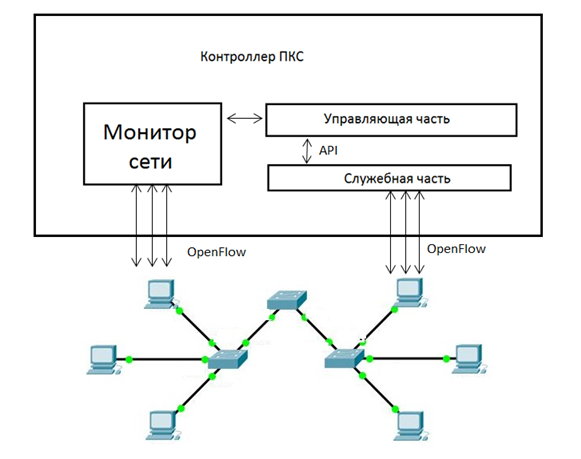
\includegraphics[width=0.8\textwidth]{scheme}
	\end{figure}

	\noindent
	Программная реализация условно делится на 3 компонента:
	\begin{enumerate}
		\item Служебная часть.
		\item Управляющая часть.
		\item Монитор сети.
	\end{enumerate}


	\subsection{Служебная часть}
	
	Служебная часть должна предоставляет управляющей:
	\begin{itemize}
		\item информацию о потоках данных, которыми обмениваются абоненты сети;
		\item информацию о проложенных в сети виртуальных каналах и их параметрах;
		\item интерфейс для добавления/удаления/модификации виртуальных каналов с определенными параметрами качества обслуживания.
	\end{itemize}

	\noindent
	Основные программные компоненты служебной части:
	\begin{itemize}
		\item Sla - класс характеристик виртуальных каналов.
		\item Vl - класс, отвечающий за хранение параметров виртуальных каналов (включая их маршруты). Также формирует набор сообщений для применения соответствующих параметров в сети.
		\item VlSet - набор виртуальных каналов.
	\end{itemize}
	
	
	\subsection{Управляющая часть}
	
	Управляющая часть:
	\begin{itemize}
		\item отвечает за построение маршрутов виртуальных каналов;
		\item отвечает за построение новых маршрутов виртуальных каналов при выходе из строя компонентов сети;
		\item использует API служебной части для применения новых маршрутов в сети после завершения работы алгоритма реконфигурации;
		\item использует информацию, полученную от монитора, для инициализации алгоритма реконфигурации.
	\end{itemize}
	
	\noindent
	Основные программные компоненты управляющей части:
	\begin{itemize}
		\item Netcontrol - класс, отвечающий за запуск алгоритма реконфигурации. Является классом приложения Runos.
		\item Algorithm - класс, реализующий алгоритмы построения маршрутов виртуальных каналов.
	\end{itemize}


	\subsection{Монитор сети}
	
	Монитор сети:
	\begin{itemize}
		\item отвечает за построение начальной топологии сети;
		\item сообщает управляющей части о выходе из строя компонентов сети.
	\end{itemize}
	
	\noindent
	Основные программные компоненты монитора:
	\begin{itemize}
		\item NetTopology - класс, отображающий текущее состояние топологии сети. Использует вспомогательные классы NetLink, NetSwitch и NetHost для хранения информации о каналах, коммутаторах и абонентах соответственно.
		\item BandwidthInfo - хранит текущую доступную на физических каналах пропускную способность. Начальные значения задаются в конфигурации приложения.
		\item HostManager - приложение Runos, анализирующее состояние абонентов. Приложение написано автором работы.
		\item SwitchManager - приложение Runos, анализирующее состояние коммутаторов. Используется стандартное приложение, входящее в состав контроллера.
		\item LinkDiscovery - приложение Runos, анализирующее состояние физических каналов. Используется стандартное приложение, входящее в состав контроллера.
	\end{itemize}


	\subsection{Начальная конфигурация сети}
	
	Конфигурация сети:
	\begin{itemize}
		\item предоставляет информацию о потоках данных между абонентами;
		\item предоставляет начальную информацию о пропускных способностях на физических каналах. В том числе пропускную способность по умолчанию;
		\item предоставляет информацию о начальном количестве коммутаторов, физических каналов и абонентов. Данная информация необходима для запуска инициализирующего алгоритма построения маршрутов виртуальных каналов.
	\end{itemize}
	
	\noindent
	Конфигурация представлена в виде xml-файла и реализована в виде класса VlConfig. \\
	Пример конфигурации:
	\lstset{ language=xml,
		%morekeywords={yield,var,get,set,from,select,partial},
		breaklines=true,
		basicstyle=\footnotesize\ttfamily}
	\linespread{1}
	\lstinputlisting{example.xml}
	
	\subsection{Общая диаграмма классов}
	Ниже представленна общая диаграмма классов, отражающая основные классы и интерфейсы, используемые для взаимодействия между ними.
	

	\section{Описание среды выполнения}
	Экспериментальная система представляет собой виртуальную среду, имитирующую функционирование:
	\begin{enumerate}
		\item Контроллера сети.
		\item Набора коммутаторов.
		\item Абонентов сети, формирующих потоки данных с заданными характеристиками.
	\end{enumerate}
	\noindent
	Виртуальная среда разворачивается на основе операционной системы Ubuntu 16.04, на которой установлены следующие компоненты:
	\begin{enumerate}
		\item Mininet – средство эмуляции сети.
		\item RUNOS – ПКС-контроллер.
		\item Ofsoftswitch13 – программный коммутатор, поддерживающий OpenFlow 1.3.
	\end{enumerate}

	\section{Инструкции по сборке}
	\subsection{Runos}
	\textbf{Начальная сборка:} \\
	C git runos. \\
	\indent
	https://github.com/ARCCN/runos/blob/master/README.md \\
	README.md той версии, которая была при разработке приложения можно найти в репозитории приложения (fork-version).[ссылка - пока что такой версии нет]
	
	\noindent
	\textbf{Сборка при внесении изменений в проект:} \\
	\indent
	cd build \\
	\indent
	make -j2
	
	\subsection{Ofsoftswitch13}
	C git ofsoftswitch. \\
	\indent
	https://github.com/CPqD/ofsoftswitch13/blob/master/README.md
	
	\subsection{Mininet}
	\indent
	http://mininet.org/download/
	
	\section{Инструкции по запуску}
	
	Порядок запуска:
	\begin{enumerate}
		\item Запустить контроллер.
		\item Запустить mininet с заданными топологией и коммутатором.
	\end{enumerate}

	\noindent
	Настройка окружения для отображения логирования: \\
	\indent
	source debug\_run\_env.sh \\
	Запуск контроллера: \\
	\indent
	build/runos \\
	Запуск топологии: \\
	\indent
	sudo mn $-$$-$custom path/topo.py $-$$-$topo mytopo $-$$-$switch user $-$$-$controller remote,port=6653
	
	
	
	
	
	
	
 
	

\end{document}
